\documentclass[12pt]{article}
\usepackage[english]{babel}
\usepackage[utf8]{inputenc}
\usepackage{graphicx}
\usepackage{float}
\usepackage[margin=1in]{geometry}
\title{CR1}
\author{Benoit Viguier}
\date{06/10/2014}
\begin{document}
\maketitle
\section{Monte Carlo Tree Search Algorithm}
\subsection{Introduction}
Monte Carlo Tree Search (MCTS) is an algorithm used for making optimal decisions in Artificial Intelligence (AI) problems such as solving games or decision making in project managment. It is based on making a big number of random simulations in order to get trustfull datas.
\subsection{How does it works ?}
The Algorithm create a tree with all possible solution with a small depth.
Then it start to run random simulations starting from the leaves in order to test the odds of the outcome.
Once we got enough the results (usually we are using time based simulations) we feed back the results and make the decision depending on the odds of each subsequent leaves.
\subsection{Example}
\label{sec:example}
\begin{figure}[H]
\centering
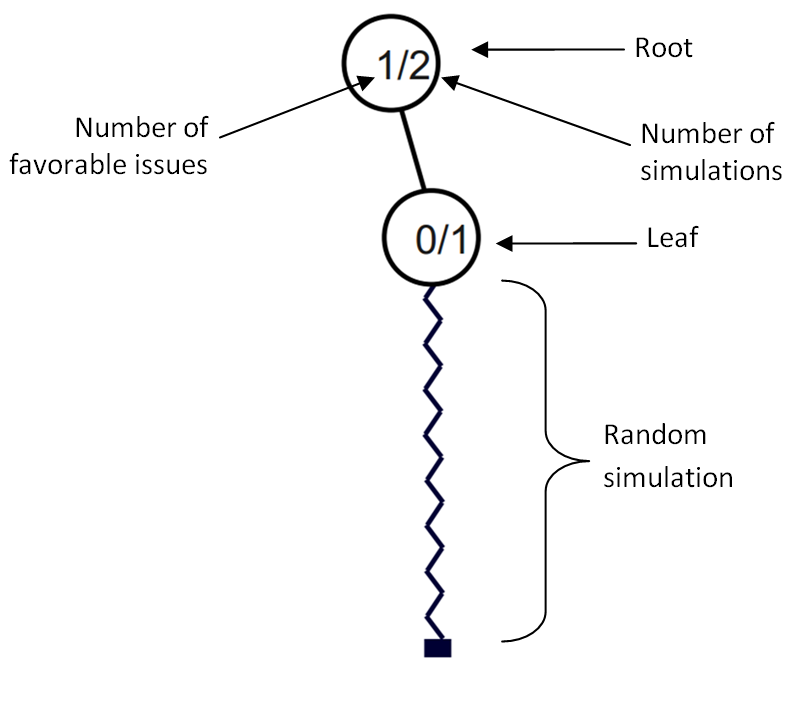
\includegraphics[height=5cm]{img/schema.png}
\caption{\label{fig:schema}Legend of the following figures.}
\end{figure}

\begin{figure}[H]
\centering
	\begin{minipage}[b]{0.45\linewidth}
		\centering
		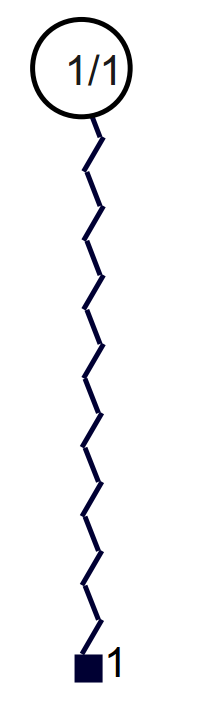
\includegraphics[height=4cm]{img/1.png}
		\caption{\label{fig:1}Run a first simulation from the root, get a favorable issue (will be considered as a \textit{win}).}
	\end{minipage}%
	\hspace*{1cm}
	\begin{minipage}[b]{0.45\linewidth}
		\centering
		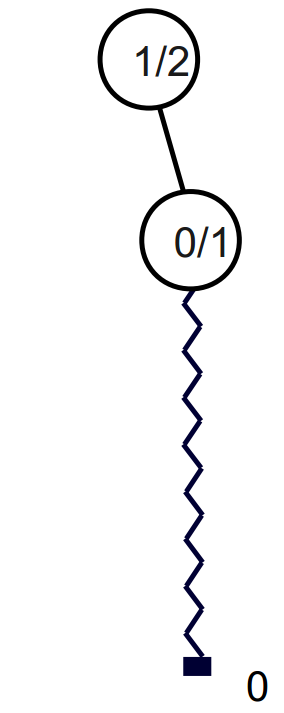
\includegraphics[height=4cm]{img/2.png}
		\caption{\label{fig:2}Create a first leaf at depth 1 and run the simulation, get an unfavorable issue (considered as a \textit{loss}).}
	\end{minipage}%
\end{figure}

\begin{figure}[H]
\centering
	\begin{minipage}[b]{0.3\linewidth}
		\centering
		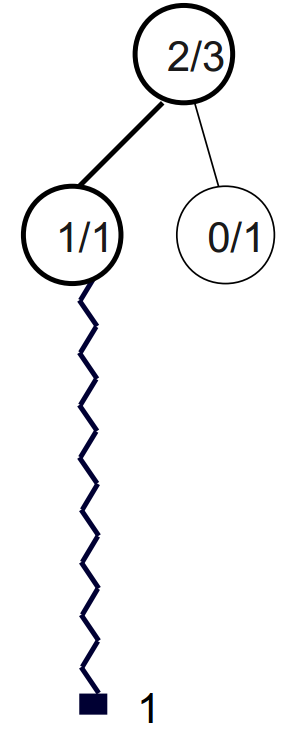
\includegraphics[height=4cm]{img/3.png}
		\caption{\label{fig:3}Create a second leaf at depth 1 and run the simulation (\textit{win}).}
	\end{minipage}%
	\hspace*{1cm}
	\begin{minipage}[b]{0.3\linewidth}
		\centering
		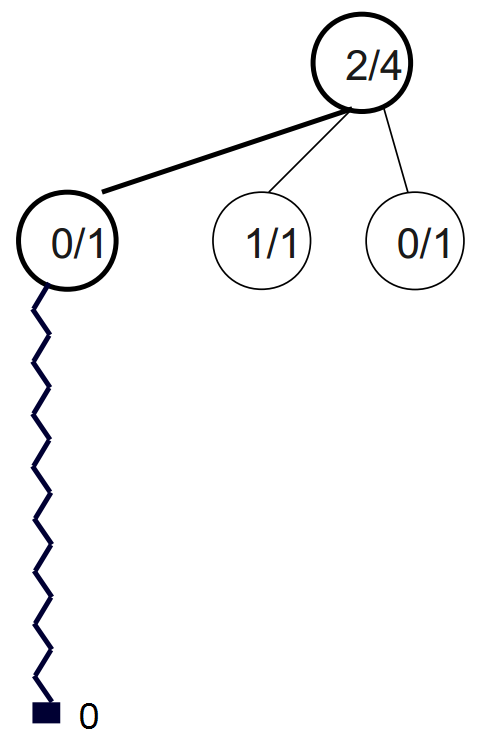
\includegraphics[height=4cm]{img/4.png}
		\caption{\label{fig:4}Create a third leaf at depth 1 and run the simulation (\textit{loss}).}
	\end{minipage}%
	\hspace*{1cm}
	\begin{minipage}[b]{0.3\linewidth}
		\centering
		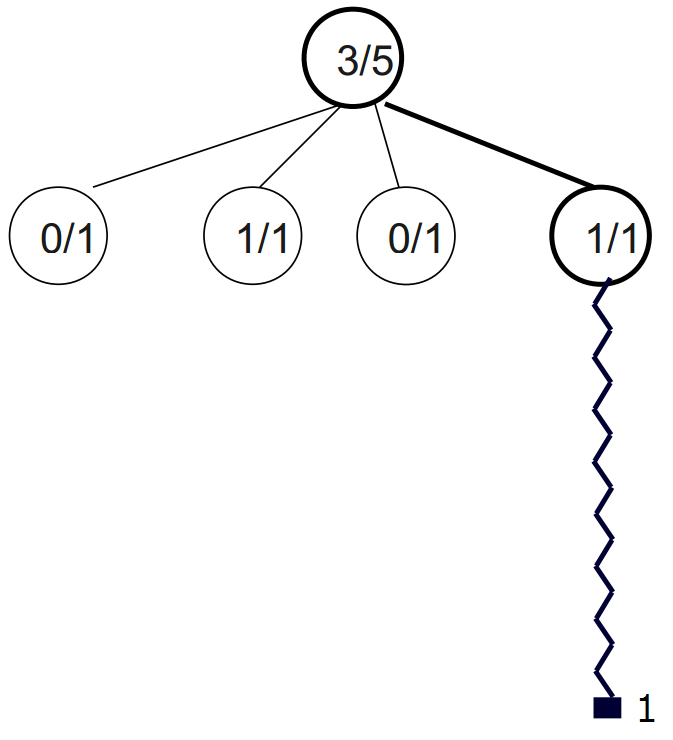
\includegraphics[height=4cm]{img/5.png}
		\caption{\label{fig:5}Create a fourth leaf at depth 1 and run the simulation (\textit{win}).}
	\end{minipage}%
\end{figure}

\noindent
Right now the odds of winning are 3/5. Now that we tested all the possible outcomes at depth 1, we will expend the tree on the favorable leaves (here the second and fourth).

\begin{figure}[H]
\centering
	\begin{minipage}[b]{0.45\linewidth}
		\centering
		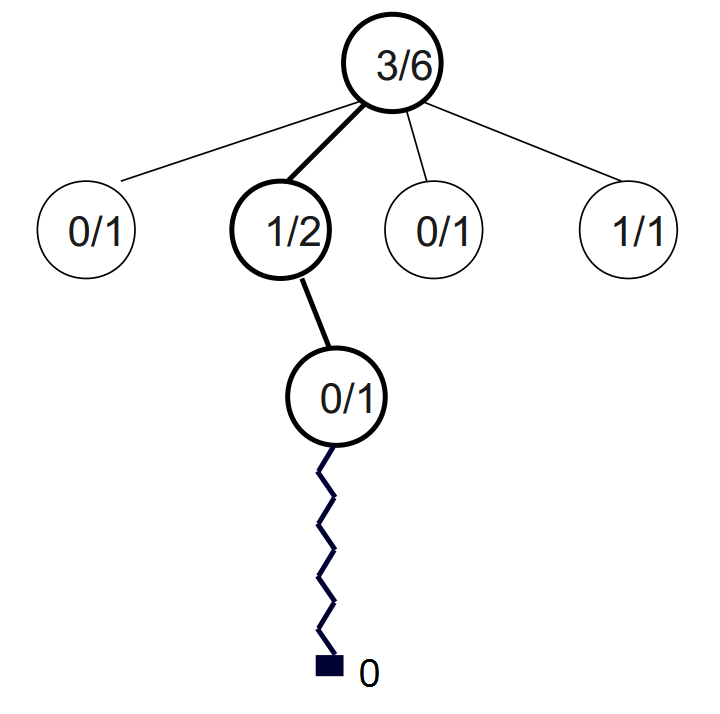
\includegraphics[height=4cm]{img/6.png}
		\caption{\label{fig:6}Create a leaf at depth 2 with parent the 2nd leaf at depth 1 and run the simulation (\textit{loss}), update the odds value of the node and making it less interesting than the fourth node. Therefore the algorithm will now work on the fourth node.}
	\end{minipage}%
	\hspace*{1cm}
	\begin{minipage}[b]{0.45\linewidth}
		\centering
		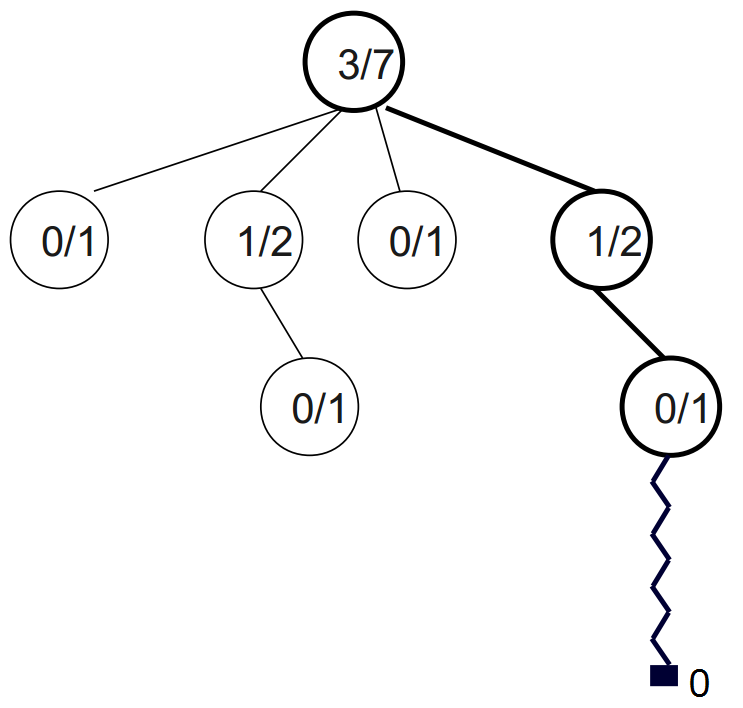
\includegraphics[height=4cm]{img/7.png}
		\caption{\label{fig:7}Create a leaf at depth 2 with parent the fourth leaf at depth 1 and run the simulation (\textit{loss}), update the odds value of the node and making it as interesting as the second node. The algorithm will now work on the second node.}
	\end{minipage}%
\end{figure}
\begin{figure}[H]
\centering
	\begin{minipage}[b]{0.45\linewidth}
		\centering
		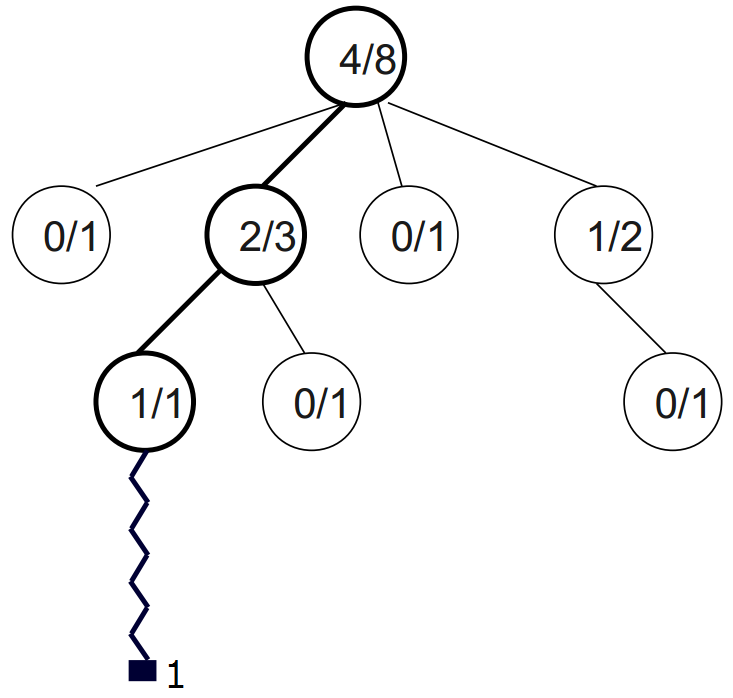
\includegraphics[height=4cm]{img/8.png}
		\caption{\label{fig:8}Create a second leaf at depth 2 with parent the second leaf at depth 1 and run simulation (\textit{win}), update the odds value and continue to develop this leaf.}
	\end{minipage}%
	\hspace*{1cm}
	\begin{minipage}[b]{0.45\linewidth}
		\centering
		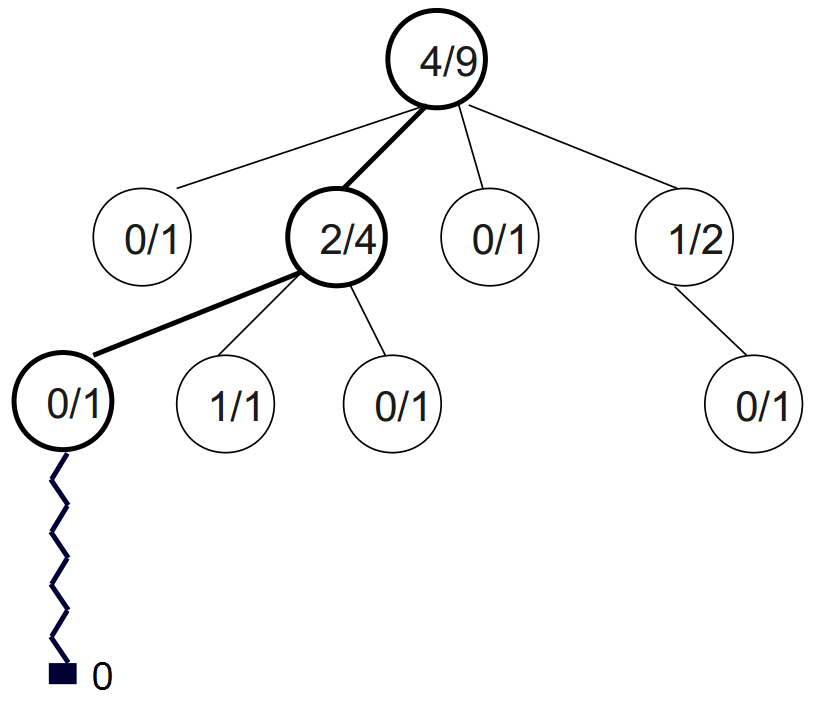
\includegraphics[height=4cm]{img/9.png}
		\caption{\label{fig:9}Create a third leaf at depth 2 with parent the second leaf at depth 1 and run simulation (\textit{loss}), update the odds value and switch to the fourth leaf.}\null\\
	\end{minipage}%
\end{figure}
\noindent
Continue the Algorithm until a decent about of simulation are run and/or the time limit is .
\begin{figure}[H]
\centering
	\begin{minipage}[b]{0.33\linewidth}
	\centering
		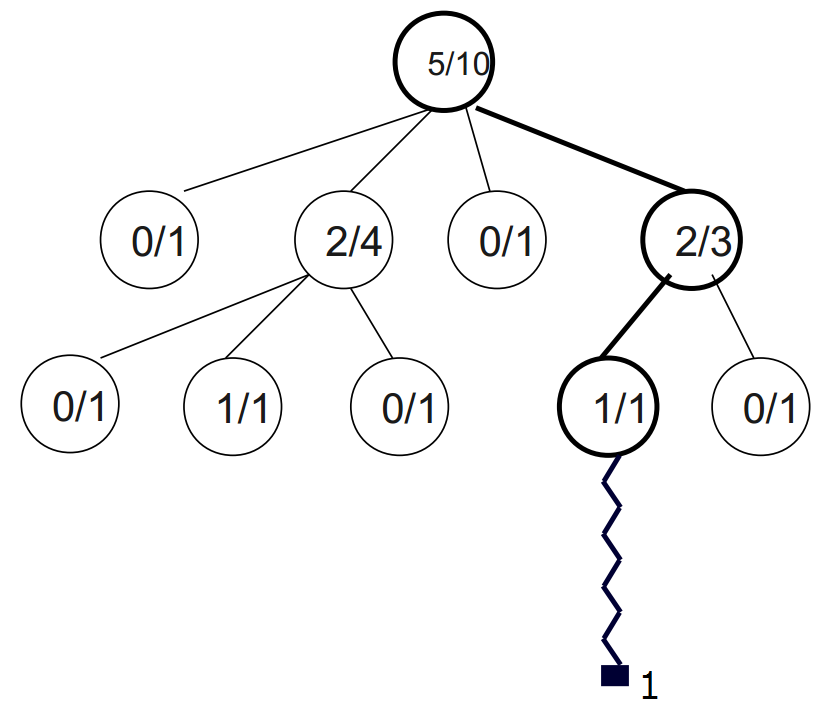
\includegraphics[height=4cm]{img/10.png}
	\end{minipage}%
	\begin{minipage}[b]{0.33\linewidth}
	\centering
		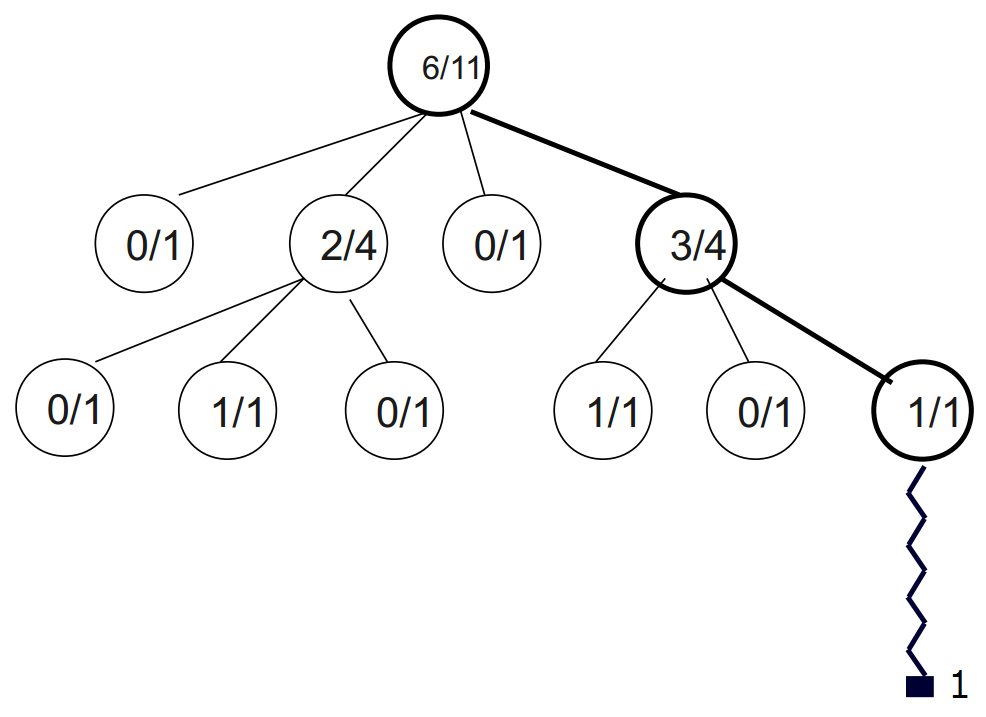
\includegraphics[height=4cm]{img/11.png}
	\end{minipage}%
	\begin{minipage}[b]{0.33\linewidth}
	\centering
		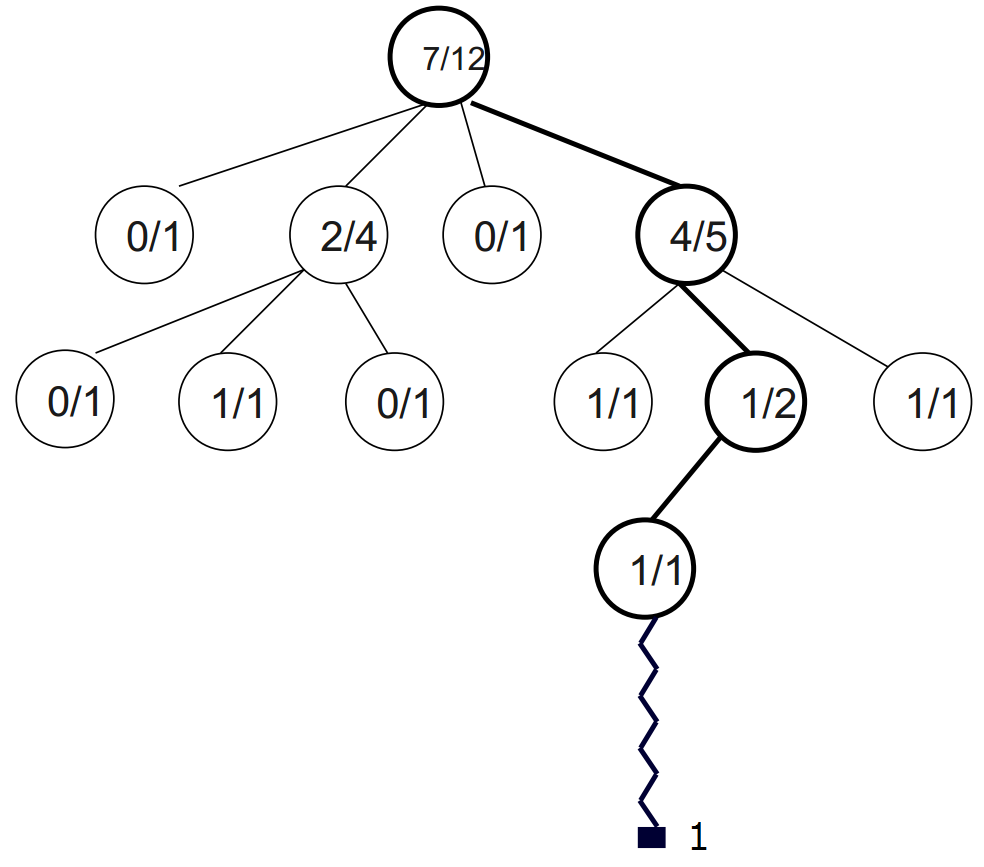
\includegraphics[height=4cm]{img/12.png}
	\end{minipage}%
\end{figure}
\noindent
Make a decision : here we chose the fourth leaf.\\
\bigskip
\subsection{How to select the leaves to develop ?}
In the previous exemple, we chose to not expend leaves without winrates. But depending on the results of the simulations, wins can vary greatly. Therefore we will run more simulations on each leaf before chosing the ones to develop. For practical purpose we will select the leaves to expend that has the highest value of the cost function UCT (Upper Confidence Bound 1 applied to Trees).\\
\bigskip
\begin{minipage}[b]{1\linewidth}
\centering
\ensuremath{f = \frac{w_i}{n_i} + c\sqrt{\frac{\ln t}{n_i}}}\\
\medskip
\tiny{\textit{UCT function}}
\end{minipage}%
\bigskip
\ensuremath{w_i} : number of wins after the ith node;\\
\ensuremath{n_i} : number of simulations after the ith node;\\
\ensuremath{c}   : exploration parameter – theoretically equal to \ensuremath{\sqrt{2}} but in practice chosen empirically;\\
\ensuremath{t}   : total number of simulations in a given tree node, equal to the sum of all \ensuremath{n_i}.\\
\medskip
The more a leaf is developed, the less it's cost is worth it. This way we can be sure that a leaf with low winrate isn't completely forgotten.\\

\subsection{Why using the Monte Carlo Tree Search ?}
Compared to other algorithm like minimax, this one is generic, once you set the rules of the games, given enough time, it will solve it. The advantage of MCTS with it's basic form is that you don't need to implement functions to improve the researches. Based on its random simulations, it will determine by itself which are the good options and which aren't.\\ The more you run simulations, the more accurate the results will be.

\subsection{How much power do we need ?}
The more the game has possible moves, the more power it require to solve. In order to get plausible decisions, it needs to go deeper in the tree and to search enough leaves. If the time or number of simulations is not sufficient, the algorithm might miss some important branches and fail to give plausible results. Therefore in order to get decent results, using high-end computer is mandatory, it allows us to get access to multi-threading technology in order to parallelize the simulations.
\end{document}